\documentclass{beamer}
\usepackage{xeCJK}
\usepackage[T1]{fontenc}
\usepackage{ifplatform}
\usepackage{mathptmx}
\usepackage{amsmath}
\usepackage{amsfonts}
\usepackage{chemformula}
\usepackage{cite}
\usepackage{graphicx}
\usepackage{hyperref}
\usepackage{minted}
\usepackage{fancyvrb}
\usepackage{etoolbox}

\defaultfontfeatures{Mapping=tex-text, Scale=MatchLowercase}
\setmainfont{Times}
\setmonofont{Times}

% Avoid ^I in minted output
\setminted{tabsize=4}



% macOS font setting
\ifmacosx
	\setCJKmainfont{Songti SC}
	\setCJKmonofont{Songti SC}
\else
% Linux and other OS font setting
	\setCJKmainfont{Source Han Sans CN}
	\setCJKmonofont{Source Han Sans CN}
\fi

% Theme
% \usetheme{metropolis}

% Information to be included in the title page:
\title{模型介绍}
\author{吴清柳}
\institute{Beijing University of Posts and Telecommunications}
\date{\today}

\begin{document}
\AtBeginSection{\tableofcontents[currentsection]}
% Title page
\maketitle

% Table of contents
\begin{frame}
	\frametitle{Table of Contentes}
	\tableofcontents
\end{frame}

\section{概述}
\begin{frame}
	\frametitle{Overview}
	通过该ppt, 对9个实验使用的模型进行介绍. 九个实验分别是鸢尾花分类实验,emojify人
	脸表情识别实验, 贷款预测, 房价预测, MNIST手写数字识别, 股票价格预测, 泰坦尼克号
	生还预测, 红酒质量预测和假新闻预测.

	使用的模型有机器学习方法如决策树, 逻辑回归, XGBoost等; 以及深度学习方法如全连接
	网络, CNN等.
\end{frame}

\section{鸢尾花分类实验}
\begin{frame}[fragile]
	\frametitle{鸢尾花分类实验}
	\begin{block}{代码和数据集}
		该论文的复现代码在\href{这里}{https://github.com/Micuks/code/blob/master/gnn/1\_iris/iris-classification/train.ipynb}
		数据集使用了鸢尾花分类数据集.
	\end{block}

	\begin{block}{模型信息}
		模型使用PyTorch编写, 为三层的全连接网络. 前两层使用ReLU激活函数, 第三层为完成分
		类功能, 使用Softmax作为激活函数, 输出分类结果.
		\begin{itemize}
			\item 第一层全连接层输入特征数量为4, 输出特征数量为25;
			\item 第二层全连接层输入特征数量为25, 输出特征数量为30;
			\item 第三层全连接层输入特征数量为30, 输出特征数量为3, 对应三类鸢尾花;
		\end{itemize}
	\end{block}
\end{frame}

\subsection{任务亮点}
\begin{frame}[fragile]{任务亮点}
	入门级任务:

	\begin{enumerate}
		\item Iris数据集简单、维度低,同时提供了一个实际的分类问题,便于初学者学习分类问题;
		\item 多类分类: 数据集包含三种不同的鸢尾花,目标是根据花的各种特征将其正确分类。
		\item 简单的特征维度: Iris数据集只有四个特征,即萼片和花瓣的长度与宽度,使得数据可视化和理解都相对容易。
		\item 明确的类别边界: 在Iris数据集中,某些类别之间的特征边界非常清晰,便于初学者进行分类.
	\end{enumerate}
\end{frame}

\subsection{数据信息}
\begin{frame}[fragile]{数据的基本信息}
	Iris数据集由英国生物学和统计学家Ronald A. Fisher在1936年提出. 数据集有150个样本, 每类花有50个样本.

	\begin{block}<only@1>{鸢尾花种类}
		鸢尾花种类有三种, 分别是:
		\begin{itemize}
			\item Iris-setosa;
			\item Iris-versicolor;
			\item Iris-virginica;
		\end{itemize}
	\end{block}
	\begin{block}{鸢尾花特征}<only@2>
		每个样本有4个特征, 单位为厘米.
		\begin{itemize}
			\item \textbf{萼片长度(sepal length)}
			\item \textbf{萼片宽度(sepal width)}
			\item \textbf{花瓣长度{petal length}}
			\item \textbf{花瓣宽度(petal width)}
		\end{itemize}
	\end{block}
	\begin{block}{目标变量}<only@2>
		目标变量是花的种类, 即前面提到的三种之一.
	\end{block}
	\begin{block}{数据分布}<only@3>
		数据集是平衡的, 意味着每个种类都有相同数量的样本(每个种类50个样本);
	\end{block}
	\begin{block}{数据清洁度}<only@3>
		鸢尾花数据集是清洁的, 没有任何的缺失值或者显著的离群值, 因此需要很少的预处理.
	\end{block}
\end{frame}

\subsection{模型介绍}
\begin{frame}[fragile]
	\frametitle{模型信息}
	模型搭建代码如下.
	\begin{minted}[breaklines]{python}
class Model(nn.Module):
def __init__(self, input_feats=4, hidden_layer1=25, hidden_layer2=30, output_feats=3) -> None:
	super().__init__()
	self.fc1 = nn.Linear(input_feats, hidden_layer1)
	self.fc2=nn.Linear(hidden_layer1, hidden_layer2)
	self.out=nn.Linear(hidden_layer2, output_feats)

def forward(self, x):
	x=F.relu(self.fc1(x))
	x=F.relu(self.fc2(x))
	x=self.out(x)

	return x
	\end{minted}
\end{frame}

\subsection{模型介绍}
\begin{frame}
	\frametitle{模型介绍}

	输入数据为鸢尾花(Iris)的特征数据. 鸢尾花有三种, 分别是Setosa, Versicolour,
	Virginica. 每个都有4个特征: sepal length, sepal width, 以及petal width.

	模型的结构介绍如下.
	\begin{block}{模型结构}
		\begin{enumerate}
			\item \textbf{输入层} 神经元数量为4, 代表4个输入特征.
			\item \textbf{第一个隐藏层`fc1'} 全连接层(dense layer), 25个神经元, 激活函数为
			      ReLU, 当输入为正时输出输入本身, 否则输出0. 如果没有非线性激活函数, 则模型将等效
			      为线性拟合函数, 拟合性能下降.
			\item \textbf{第二个隐藏层`fc2'} 另一个全连接层, 30个神经元, 激活函数为ReLU;
			\item \textbf{输出层`out'} 一个全连接层, 3个神经元, 对应鸢尾花的三个分类:
			      Setosa, Versicolour, Virginica.
		\end{enumerate}
	\end{block}

\end{frame}

\subsection{训练方法}
\begin{frame}[fragile]
	\frametitle{训练方法}
	使用交叉熵作为损失函数, Adam为优化器, 学习率为0.01, 在训练集上进行100轮训练. 对loss可视化观察后看到大约40轮后模型已经接近收敛.
	\begin{block}{训练代码}
		\begin{minted}[breaklines=true]{python}
epochs=100
losses=[]
for i in range(epochs):
    y_pred=model.forward(X_train)
    loss=criterion(y_pred,y_train)
    losses.append(loss)
    print(f'epoch: {i:2} loss: {loss.item():10.8f}')
    
    optimizer.zero_grad()
    loss.backward()
    optimizer.step()
	\end{minted}
	\end{block}
\end{frame}

% Slide 1: Introduction to Training Duration and Loss Storage
\begin{frame}[fragile]
	\frametitle{初始化}
	\begin{itemize}
		\item 一轮代表对所有训练样本的一个完全的前向传播和反向传播过程;
		\item \texttt{losses}列表会存储在每轮中计算的loss值, 用于追踪模型的表现;
	\end{itemize}
	\begin{minted}[breaklines]{python}
		epochs = 100
		losses = []
		\end{minted}
\end{frame}

% Slide 2: The Training Loop - Forward Pass and Loss Calculation
\begin{frame}[fragile]
	\frametitle{训练循环: 前向传播和损失计算}
	Within the loop, the model predicts outcomes and computes the discrepancy between predictions and actual values.
	在训练循环中, 模型预测输出, 计算预测值和实际值之间的差异;

	\begin{minted}[breaklines]{python}
for i in range(epochs):
    y_pred = model.forward(X_train)
    loss = criterion(y_pred, y_train)
    losses.append(loss)
\end{minted}
\end{frame}

% Slide 3: The Training Loop - Logging, Backward Pass, and Optimization
\begin{frame}[fragile]
	\frametitle{训练循环: 日志和优化}
	\begin{itemize}
		\item 通过打印轮数和loss值来监控训练进程;
		\item 计算梯度并更新模型参数来降低loss;
	\end{itemize}

	\begin{minted}[breaklines]{python}
    print(f'epoch: {i:2} loss: {loss.item():10.8f}')
    optimizer.zero_grad()
    loss.backward()
    optimizer.step()
\end{minted}
\end{frame}

\section{Emojify表情识别实验}
\begin{frame}
	\frametitle{利用CNN进行面部表情识别}

	在该实验中, 利用Tensorflow来搭建CNN网络进行对摄像头采集的人脸进行表情识别. 模型使用
	GPU进行训练, 得到的权重文件作为表情识别的依据.

	此处使用Tensorflow是为了将Pytorch和Tensorflow两个常用框架都进行学习.

\end{frame}

\subsection{任务亮点}
\begin{frame}[fragile]{任务亮点}
	\begin{enumerate}
		\item \textbf{实时应用场景} 借助Tensorflow训练完成后, 导出的权重文件可以实时对摄像头画面进行标签识别.
		\item \textbf{深度学习应用} 借助卷积神经网络(CNN)为面部表情分类这一图像任务提供了强有力的帮助, 这是因为CNN特别擅长捕捉图像数据中的层次结构和模式.
		\item \textbf{多分类问题} 面部情感识别通常包括多个类别, 例如快乐, 悲伤, 惊讶, 愤怒等, 增加了任务的复杂型.
	\end{enumerate}
\end{frame}
\subsection{数据基本信息}
\begin{frame}[fragile]{数据基本信息}
	使用FER2013数据集.
	\begin{enumerate}
		\item<only@1> \textbf{数据来源} FER2013是为了2013年ICML举办的情感识别挑战而创建的. 该数据集在Kaggle上发布, 旨在为面部情感识别任务提供一个标准化的挑战.
		\item<only@1> \textbf{样本数量} 数据集包含35,887张图像.
		\item<only@1> \textbf{数据类型} 灰度图像. 相比于彩色图像, 灰度图像可以减少计算复杂型, 且足够进行表情识别;
		\item<only@1> \textbf{图像大小} 图像大小为$48\times 48$像素.
		\item<only@2> \textbf{类别/标签} 数据集包括七个面部表情标签:
			\begin{itemize}
				\item 0=Angry(愤怒)
				\item 1=Disgust(厌恶)
				\item 2=Fear(恐惧)
				\item 3=Happy(高兴)
				\item 4=Sad(悲伤)
				\item 5=Surprise(惊讶)
				\item 6=Neutral(中性)
			\end{itemize}
		\item<only@2> \textbf{数据分割} 在本次实验中, FER2013被分为三个子集:
			\begin{itemize}
				\item \textbf{训练集 } 有28,709个样本;
				\item \textbf{验证集 } 有3,589个样本, 用于训练过程中验证;
				\item \textbf{测试集 } 有35,89个样本, 用于最终的测试评估;
			\end{itemize}
		\item<only@3> \textbf{数据不均衡问题 } 数据集中某些情感的样本数量比其他情感多. 例如, ``Happy''表情的样本数量远多于``Disgust''.
		\item<only@3> \textbf{挑战性 } 由于图像是灰度的, 并且分辨率较低($48\times 48$), 因此识别模型需要能够从较少的信息中捕获细微的面部特征.
	\end{enumerate}
\end{frame}

\subsection{模型介绍}
% Slide 1: Introduction to the Model
\begin{frame}[fragile]
	\frametitle{CNN模型结构}
	\begin{itemize}
		\item 目的: 从灰度图片进行表情识别;
		\item 图片输入形状: \(48 \times 48 \times 1\);
		\item 层之间顺序堆叠;
	\end{itemize}
	\begin{minted}[breaklines]{python}
emotion_model = Sequential()
\end{minted}
	Keras中的`Sequential'是层之间的线性堆叠. 可以允许我们来通过将层逐个堆叠来搭建神经网络.
\end{frame}

% Slide 2: Initial Convolution Layers
\begin{frame}[fragile]
	\frametitle{初始化卷积层}
	\begin{minted}[breaklines]{python}
emotion_model.add(
    Conv2D(32, kernel_size=(3, 3), activation="relu", input_shape=(48, 48, 1))
)
emotion_model.add(Conv2D(64, kernel_size=(3, 3), activation="relu"))
emotion_model.add(MaxPooling2D(pool_size=(2, 2)))
emotion_model.add(Dropout(0.25))
\end{minted}
	\only<1>{\begin{block}{第一个卷积层}
			第一个卷积层有32个卷积核, 每个尺寸为$3\times 3$, 来处理尺寸为$48\times 48$的输
			入图片. `relu'激活函数引入了非线性, 让模型可以捕获复杂的特征.
		\end{block}}
	\only<2>{\begin{block}{第二个卷积层}
			第二个卷积层有64个$3\times 3$的卷积核, 该层进一步处理了来自前一层的特征图, 检测了输入图片中的更复杂的特征.
		\end{block}}
	\only<3>{\begin{block}{Max-Pooling层}
			该层通过从每个$2\times 2$窗口中取最大值来对特征图进行降采样. 这减少了计算负担, 并帮助让模型平移不变.
		\end{block}}
	\only<4>{\begin{block}{Dropout层}
			Dropout可以用来避免过拟合. 0.25的Dropout率意味着大约25\%的神经元在前面的层会被随
			机在训练中关闭, 使得可以获得容错率更高的模型.
		\end{block}}
\end{frame}

% Slide 3: Deeper Convolution Layers
\begin{frame}[fragile]
	\frametitle{多个卷积层}
	\begin{minted}[breaklines]{python}
emotion_model.add(Conv2D(128, kernel_size=(3, 3), activation="relu"))
emotion_model.add(MaxPooling2D(pool_size=(2, 2)))
emotion_model.add(Conv2D(128, kernel_size=(3, 3), activation="relu"))
emotion_model.add(MaxPooling2D(pool_size=(2, 2)))
emotion_model.add(Dropout(0.25))
\end{minted}
	\only<1>{\begin{block}{更深的卷积层}
			后面的具有128个卷积核的卷积层每个都进一步细化了特征图. 随着模型变深, 这些层会捕获图片中更多的高层特征.

			每个卷积层后面都有一个Max-Pooling层来降采样, 降低计算负担, 提高平移不变性.
		\end{block}}
\end{frame}

% Slide 4: Fully Connected Layers
\begin{frame}[fragile]
	\frametitle{全连接层}
	\begin{minted}[breaklines]{python}
emotion_model.add(Flatten())
emotion_model.add(Dense(1024, activation="relu"))
emotion_model.add(Dropout(0.25))
emotion_model.add(Dense(7, activation="softmax"))
\end{minted}

	\only<1>{\begin{block}{Flatten扁平化层}
			该层将2D的特征矩阵映射到1D的向量. 在将数据传入全连接层之前, 这是必要的步骤;
		\end{block}}
	\only<2>{\begin{block}{稠密全连接层}
			具有1024个神经元的全连接层允许模型来基于由卷积层提取的高层次特征来进行决策. `ReLU'激活函数确保了非线性.
		\end{block}}
	\only<3>{\begin{block}{输出层}
			输出稠密层有7个神经元, 对应在数据集中的七种表情分类. `softmax'激活函数确保了输出值是和为1的概率.
		\end{block}}
	\only<4>{\begin{block}{Softmax}
			Softmax函数常常被用在基于神经网络的分类器的最后一层, 将一个实数向量转化为一个概
			率分布.

			在数学上, 对一个向量$z$的Softmax函数$\sigma$可以被定义为
			\begin{equation}
				\sigma(z)_i=\frac{e^{z_i}}{\sum^K_{j=1}{e^{z_j}}}
			\end{equation}
			其中,
			\begin{itemize}
				\item $\sigma(z)_i$是$z$的第$i^{th}$个分量的Softmax函数输出;
				\item $K$是分类的数量(也是向量$z$的长度);
			\end{itemize}
		\end{block}}
	\only<5>{\begin{block}{Softmax}
			指数函数确保了输出向量所有的分量都是非负的, 除法将所有的分量规范化, 让他们的和为
			1. 结果向量因此可以表示$K$个类别的概率分布.
		\end{block}}
	\only<6>{\begin{block}{为什么使用Softmax}
			\begin{enumerate}
				\item \textbf{概率解释} softmax函数被用于分类模型的输出层, 因为他提供了多个类之
				      间的概率分布. 这意味着对于给定的输入, 模型可以提供输入可能属于哪个输出的类别;
				\item \textbf{处理多个类 }在分类问题中, 尤其是对于超过两个类别的情况, 分类时需要
				      不仅知道哪个类是最可能属于的, 还想预测和其他类的似然成都. Softmax可以通过将每个
				      类的输出压缩在0和1之间, 并确保他们的和为1来帮助实现这一目标.
				\item \textbf{基于梯度的优化} Softmax与类别交叉熵作为loss函数, 提供了一个表现良
				      好的梯度. 在训练神经网络的反向传播阶段非常有用. 没有良好的梯度, 神经网络将不能高效的学习.
			\end{enumerate}
		\end{block}}
\end{frame}

\begin{frame}[fragile]{Cross-Entropy}
	Cross-entropy是衡量两个概率分布之间的差异的方法. 在机器学习和深度学习中, 它常常
	被用作损失函数来量化预测概率分布和真实分布之间的差异.

	对两个离散的概率分布$p$和$q$, 交叉熵$H(p,q)$被定义为
	\begin{equation}
		H(p,q)=-\sum_x{p(x)\log{(q(x))}}
	\end{equation}
	其中,
	\begin{itemize}
		\item $p(x)$是事件$x$发生的真实概率;
		\item $q(x)$是事件$x$发生的预测概率;
		\item 对于所有的可能事件$x$进行求和;
	\end{itemize}

	对于用于分类任务的神经网络, $p$是真实标签的独热编码向量, $q$是预测概率(经常通过
	softmax函数取得).
\end{frame}

\begin{frame}
	\frametitle{为什么使用Cross-entropy}

	\begin{enumerate}
		\item \textbf{概率解释 } Cross-entropy提供了真实概率分布和预测概率分布之间的差异
		      的度量. 较低的交叉熵值表明模型的预测与真实标签比较相似.
		\item \textbf{可微分 } 对于学习算法, 尤其是神经网络, 具有一个可微分的损失函数是
		      至关重要的. 交叉熵可微分, 使得他可以被用于像梯度下降这样的基于梯度的优化方法.
		\item \textbf{惩罚自信的错误预测 } 交叉熵作为loss函数的一个优点是它如何处理预测.
		      如果一个模型对一个错误的类别预测0.99的概率, 对正确的类别预测0.01的概率, 交叉熵会
		      变得非常大. 这个特征确保了当模型非常自信得犯错的时候, 会被严重惩罚;
		\item \textbf{和Softmax配合良好} 交叉熵损失结合输出层中的softmax激活函数是分类问
		      题中流行的组合. 从这个组合中获得的梯度有良好的属性, 使得模型可以更快收敛, 并且经
		      常相较于其他的激活函数-损失函数对具有更好的解决方案.
		\item \textbf{解决饱和问题 } 在神经网络中, sigmoid激活函数和quadratic cost可以导
		      致``饱和''问题, 此时神经元的输出和梯度都几乎是0, 使得网络难以训练. 交叉熵不会受
		      这个问题困扰, 使得训练更加高效.
	\end{enumerate}

\end{frame}

\subsection{模型训练}
\begin{frame}[fragile]
	\frametitle{模型训练}

	神经网络模型的结构确定后, 下一个关键步骤就是在数据上对其进行训练.

	\begin{enumerate}
		\item<1-> \textbf{编译模型}
			\only<1>{
				\begin{itemize}
					\item \textbf{损失函数 } 模型使用`categorical\_crossentropy'作为损失函数.
					\item \textbf{优化器 } 使用`Adam'作为优化器. Adam对每个参数调节学习率. 其具有高
					      效率与低内存需求. `learning\_rate'战术决定了优化器最小化loss的步长, `decay'可以
					      随时间降低学习率来允许在之后的训练过程中更细化的权重更新.
					\item \textbf{矩阵 } `accuracy'是在训练过程中监控的矩阵. 准确率提供了一个清晰的,
					      直观的对模型执行情况的理解: 表示正确分类的实例在总实例中占的百分比.
				\end{itemize}}
		\item<2-> \textbf{拟合模型 }
			\only<2>{
				\begin{itemize}
					\item \textbf{数据源 } 模型借助`fit\_generator'方法进行训练, 该方法允许边读取边
					      数据增强(data augmentation on-the-fly), 且更加内存高效. 该方法当训练集太大而无法
					      整个放入内存的时候更合适.
					\item \textbf{轮数 } 模型训练了50轮. 每轮代表一次对于所有训练样本的前向传播和反
					      向传播.
					\item \textbf{Batch Size } 每一轮的步数(`28709 // 64')表示数据每次被传入大小为64
					      个实例的批次. 类似的, 对于验证阶段, 使用批次大小`7178 // 64'. 使用批次加速了训练
					      过程, 因为模型权重的更新是在每一轮后进行的, 而不是在每个数据点之后.
					\item \textbf{验证数据 }模型的表现在一个单独的验证数据几上并行验证. 这帮助了监控
					      任何的过拟合信号, 当模型在训练数据上表现异常良好, 而对于新的没有见过的数据非常糟糕的时候就发生了过拟合.
				\end{itemize}}
	\end{enumerate}

\end{frame}

\section{贷款预测}
\begin{frame}
	\frametitle{使用逻辑回归模型的贷款预测}

	借助scikit-learn的逻辑回归模型对是否可以给用户贷款进行预测. 该实验主要内容在于数
	据预处理.

\end{frame}

\subsection{任务介绍}
\begin{frame}[fragile]{贷款预测任务介绍}
	金融机构放贷需要评估借款人违约的风险, 从而降低坏账损失, 确保资金安全. 该任务通过逻辑回归来预测是否可以放贷.

	\begin{block}{二分类问题}
		借贷问题是一个二分类问题, 目标是预测借款人是否会还款. 输出通常是`yes'或`no'.
	\end{block}

	对该问题, 在数据预处理上要使用特征工程来判断哪些信息结合可以作为比较良好的放贷参照. 例如, 将收入和负债比进行组合等.

	对该问题使用逻辑回归, 是因为逻辑回归不仅可以提供预测结果, 还可以为每个预测提供概率评分. 这有助于评估违约的风险程度.
\end{frame}

\begin{frame}[fragile]{贷款预测任务介绍}
	\begin{block}{可解释性}
		与深度学习模型相比, 逻辑回归的一个主要优势是其可解释性. 在信贷审批过程中, 理解为什么某个请求被拒绝或者批准是重要的, 逻辑回归的系数可以提供有关哪些特征最影响预测的见解.
	\end{block}
	\begin{block}{应对不平衡数据}
		信贷数据通常是不平衡的, 因为违约的案例可能远远少于正常偿还的案例. 因此需要使用特定的方法, 例如过采样, 欠采样等方法来解决.
	\end{block}
\end{frame}

\subsection{数据介绍}
\begin{frame}[fragile]{数据集基本信息}
	\begin{block}{数据来源}<only@1>
		来源于kaggle社区的公开数据集``Loan Prediction Problem''.
	\end{block}
	\begin{block}{特征}<only@1>
		数据集包含多个特征, 例如申请人的性别, 婚姻情况, 教育程度, 受雇状态, 收入, 贷款金额和信贷历史.
	\end{block}
	\begin{block}{目标变量}<only@1>
		`Loan\_Status'是目标变量, 是二元变量. 其中`Y'表示贷款获得批准, `N'表示贷款没有获得批准.
	\end{block}
	\begin{block}{数据规模}<only@1>
		训练集大小为$614\times 13$, 测试集大小为$367\times 12$. 其中测试集少了`Loan\_Status'一栏.
	\end{block}
\end{frame}

\begin{frame}[fragile]{数据集特征}
	数据集有如下特征:
	\begin{itemize}
		\item Loan\_ID: 一个单独的标识数字, 每个申请人独有;
		\item Gender: 性别(男/女);
		\item Married: 申请人是否结婚(Yes/No);
		\item Dependents: 申请人的家人数量, 0/1/2/3+.
		\item Education: 教育等级(已毕业/未毕业);
		\item Self\_Employed: 是否申请人是自雇人士(是/否);
		\item ApplicantIncome: 申请人收入;
		\item CoapplicantIncome: 共同申请人收入(如果没有共同申请人则为0);
		\item LoanAmount: 申请的贷款金额(千为单位);
		\item Loan\_Amount\_Term: 贷款期限(月为单位);
		\item Credit\_History:借款人负责偿还债务的记录, 为0或1, 表示申请人是否有过贷款偿还历史;
		\item Property\_Area:申请贷款的房产所在的区域类型(城市/半城市/农村);
	\end{itemize}
\end{frame}

\subsection{模型训练和预测}
\begin{frame}[fragile]{模型训练和预测}
	\begin{minted}[breaklines,tabsize=4]{python}
LR=LogisticRegression()
LR.fit(X_train,y_train)
y_hat=LR.predict(X_test)

# prediction summary by species
print(classification_report(y_test,y_hat))

# accuracy score
LR_SC=accuracy_score(y_hat,y_test)
print('accuracy is',accuracy_score(y_hat,y_test))
\end{minted}
\end{frame}

\begin{frame}[fragile]{逻辑回归}
	`Logistic Regression'是一个用来进行二元分类问题的统计方法, 一个分类问题指预测一
	个特定数据属于两个中的哪一个类. 被叫做``logistic'' 回归因为是基于逻辑函数的, 这
	被用于建模将一个给定的输入点划入两个分类之一的概率.
\end{frame}

\begin{frame}[fragile]{训练模型}
	\begin{minted}[breaklines,tabsize=4]{python}
LR=LogisticRegression()
LR.fit(X_train,y_train)
\end{minted}
	\begin{itemize}
		\item 首先, 借助`LogisticRegression()'来获取一个逻辑回归模型.
		\item 下一步, `fit'方法将模型在训练数据上进行训练. 这里, `X\_train'是具有特征的
		      训练数据, `y\_train'是训练数据对应的标签.
	\end{itemize}
\end{frame}

\begin{frame}[fragile]{进行预测}
	\begin{minted}[breaklines,tabsize=4]{python}
y_hat=LR.predict(X_test)
	\end{minted}
	在将模型在训练数据上训练后, 下一步就是在新的没有见过的模型上进行预测. `predict'
	方法将测试数据`X\_test'作为参数, 返回预测标签`y\_hat'.
\end{frame}

\begin{frame}[fragile]{分类报告}
	\begin{minted}[breaklines,tabsize=4]{python}
	print(classification_report(y_test,y_hat))
	\end{minted}
	`classification\_report'提供了模型表现的准确度, 召回度和F1-score.
	\begin{itemize}
		\item \textbf{Precision准确度}
		      在所有预测为某个特定类的例子中, 多少是真阳性;

		\item \textbf{Recall召回率}
		      在所有属于一个特定类的实例中, 哪些被正确预测了, 即真阳性与真阴性的和;

		\item \textbf{F1-score}
		      准确度和召回率的调和平均值, 提供了两个之间的平衡指标.

	\end{itemize}
\end{frame}

\begin{frame}[fragile]{Precision准确度}
	\begin{equation}
		\text{Precision}=\frac{\text{True Positives}}{\text{True Positives}+\text{False Positives}}
	\end{equation}

	当假阳性的代价高的时候, 准确度是关键的.
\end{frame}

\begin{frame}[fragile]{Recall召回率}
	\begin{equation}
		\text{Recall}=\frac{\text{True Positives}}{\text{True Positives}+\text{False Negatives}}
	\end{equation}

	当假阴性的代价高的时候, 召回率是重要的.
\end{frame}

\begin{frame}[fragile]{准确率分数}
	\begin{minted}[breaklines,tabsize=4]{python}
LR_SC=accuracy_score(y_hat,y_test)
print('accuracy is',accuracy_score(y_hat,y_test))
	\end{minted}

	准确率分数是一个可以表明在测试数据中正确预测的分类的占比的量. 计算方式为将正确预
	测的数量除以预测的总数.
	\begin{equation}
		\text{Accuracy}=\frac{\text{Number of correct predictions}}{\text{Total number of predictions}}
	\end{equation}

	对于本处的贷款预测:
	\begin{itemize}
		\item 如果一个贷款请求倾向于被允许, 模型会预测`1', 否则为0.
		\item 准确率通过将预测结果与实际情况对比告诉我们多少的贷款请求被我们的模型正确预测.
	\end{itemize}

\end{frame}
\subsection{模型局限}
\begin{frame}[fragile]{模型局限}
	逻辑回归具有这样的局限:
	\begin{description}
		\item[线性决策边界] 逻辑回归假设一个线性决策边界, 这可能不能捕获数据中的复杂关系.
		\item[特征的独立性] 逻辑回归假设输入特征是独立的, 意味着他们不会互相影响. 如果一
			些特征是强相关的, 这可能影响模型的参数.
	\end{description}
\end{frame}

\section{房价预测}
\begin{frame}[fragile]{在Boston Hosting数据集上进行房价预测}
	借助PyTorch搭建全连接模型对Boston Hosting数据集进行房价预测.
\end{frame}

\subsection{模型结构}
\begin{frame}[fragile]{模型结构}
	\begin{minted}[breaklines,tabsize=4]{python}
	# boston housing model
class BostonHousingModel(nn.Module):
    def __init__(self):
        super(BostonHousingModel,self).__init__()
        self.layer1=nn.Linear(13,64)
        self.layer2=nn.Linear(64,64)
        self.layer3=nn.Linear(64,1)
        
    def forward(self,x):
        x=torch.relu(self.layer1(x))
        x=torch.relu(self.layer2(x))
        x=self.layer3(x)
        return x
	\end{minted}
	模型借助PyTorch框架, 使用`nn.Module'基类来定义神经网络结构.
\end{frame}

\begin{frame}[fragile]{模型初始化}
	\only<1>{\begin{block}{第一层}
			全连接层, 输入特征为13, 对应Boston Housing dataset中的13个特征, 输出特征数量为64.
		\end{block}}
	\only<1>{\begin{block}{第二层}
			全连接层, 输入特征数量为64, 输出特征数量为64.
		\end{block}}
	\only<1>{\begin{block}{第三层}
			全连接层, 输入特征数量为64, 输出特征数量为1, 即表示预测房价结果.
		\end{block}}
\end{frame}

\begin{frame}[fragile]{前向传播}
	前向传播方法描述了输入数据是如何流过模型的.
	\begin{itemize}
		\item \textbf{第一步 }将输入`x'通过`layer1', 应用ReLU(Rectified Linear Unit)激活
		      函数. ReLu函数引入非线性, 允许模型从错误中学习和调整, 对于学习复杂的特征至关重
		      要;
		\item \textbf{第二步 }将前一步的输出传入`layer2', 再次使用ReLU激活函数;
		\item \textbf{最后一步 }将结果传过`layer3'. 在这一层没有激活函数, 因为这是一个回
		      归问题, 模型被设计为直接输出连续值.
	\end{itemize}
\end{frame}

\begin{frame}[fragile]{模型训练}
	\begin{itemize}
		\item \textbf{损失函数 } 使用`nn.MSELoss()'作为损失函数. 平均平方差损失计算了预
		      测和实际值的平均平方差, 对于房价预测问题是合适的选择.
		\item \textbf{优化器选择 } 选择Adam优化器来调节模型参数. 学习率为`0.001'.
		\item \textbf{训练轮数 } 训练500轮, 并记录日志.
	\end{itemize}
\end{frame}

\subsection{改进模型}

\begin{frame}[fragile]{改进模型}
	在前面基础模型的基础上, 使用Dropout进行改进. 在训练策略上, 使用学习率规划下降和提前停止来优化训练.
	\begin{minted}[breaklines,tabsize=4]{python}
class OptiBostonHousingModel(nn.Module):
    def __init__(self):
        super(OptiBostonHousingModel,self).__init__()
        self.layer1=nn.Linear(13,128)
        self.layer2=nn.Linear(128,64)
        self.dropout=nn.Dropout(0.5)
        self.layer3=nn.Linear(64,1)
        
    def forward(self,x):
        x=torch.relu(self.layer1(x))
        x=self.dropout(x)
        x=torch.relu(self.layer2(x))
        x=self.dropout(x)
        x=self.layer3(x)
        return x
	\end{minted}
\end{frame}

\begin{frame}[fragile]{模型结构}
	仍旧是三层全连接层, 但是第二层和第三层之间使用了Dropout率为0.5的dropout层, 随机
	丢弃一半输入数据来帮助避免过拟合.

	\begin{block}{学习率规划器}
		使用`StepLR'规划器来在训练过程中调节学习率. 特别的, 学习率每100轮被乘以一个参数
		`gamma'(此处为0.1). 随时间降低学习率可以帮助细化模型的权重, 使其更加贴近最优方案.
	\end{block}
\end{frame}

\section{MNIST手写数字识别}
\begin{frame}[fragile]{CNN进行MNIST手写数字识别}
	借助PyTorch框架, 定义一个CNN进行MNIST手写数字识别.
\end{frame}

\subsection{模型结构}
\begin{frame}[fragile]{模型结构}
	\begin{minted}[breaklines,tabsize=4]{python}
class CNN(nn.Module):
    def __init__(self):
        super(CNN, self).__init__()

        self.conv_layers = nn.Sequential(
            # (n, 1, 28, 28) -> (n,32,28,28)
            nn.Conv2d(1, 32, kernel_size=3, stride=1, padding=1),
            nn.ReLU(),
            # (n,32,28,28)->(n,32,14,14)
            nn.MaxPool2d(kernel_size=2, stride=2),
            # (n,32,14,14)->(n,64,14,14)
            nn.Conv2d(32, 64, kernel_size=3, stride=1, padding=1),
            nn.ReLU(),
            # (n,64,14,14)->(n,64,7,7)
            nn.MaxPool2d(kernel_size=2, stride=2),
        )
	\end{minted}

\end{frame}
\begin{frame}[fragile]
	\frametitle{模型结构}

	\begin{minted}[breaklines,tabsize=4]{python}
        self.fc_layers = nn.Sequential(
            # (n,64*7*7)->(n,128)
            nn.Linear(64 * 7 * 7, 128),
            nn.ReLU(),
            # (n,128)->(n,10)
            nn.Linear(128, 10),
        )

    def forward(self, x):
        x = self.conv_layers(x)
        x = x.view(x.size(0), -1)  # flatten the tensor
        x = self.fc_layers(x)
        return x
	\end{minted}

\end{frame}

\begin{frame}[fragile]{模型结构}
	\begin{enumerate}
		\item<only@1> \textbf{卷积层(`conv\_layers')}
			这些层用来处理输入图像的空间信息, 检测局部图案, 边缘, 纹理等. 通过级联卷积和池化操作以分层方式转换图像.
			\begin{enumerate}
				\item \textbf{第一卷积层}
				      \begin{itemize}
					      \item \textbf{卷积 } 这一层使用单个通道(因为MNIST图片为灰度图片), 将其转化为32个通道, 借助$3\times 3$卷积核. 大小为1的填充确保了输出和输入的宽和高相同, 因此输出形状为$(n,32,28,28)$.
					      \item \textbf{激活函数 } `ReLU'激活函数引入了非线性.
					      \item \textbf{池化 } 之后的`MaxPool2d'操作使用了步长为2的池化核大小为$2\times 2$
					            的池化操作来降低空间维度大小到原来的一半, 使得输出形状为$(n,32,14,14)$.
				      \end{itemize}
				\item \textbf{第二卷积层}
				      \begin{itemize}
					      \item 卷积: 将前一层的32个通道借助$3\times 3$的卷积核转化为64通道, 由于填充为1, 保留了原本的维度.
					      \item 激活函数: ReLU.
					      \item 池化: 另一个`MaxPool2d'操作将其维度降低到原来的一半, 输出形状为$(n,64,7,7)$.
				      \end{itemize}
			\end{enumerate}
		\item<only@2> \textbf{全连接层(`fc\_layers')}
			\begin{itemize}
				\item 这些层分析卷积层提取和学到的特征, 将其分类到10个可能的数字类中.
			\end{itemize}
			\begin{enumerate}
				\item \textbf{第一个全连接层 }
				      \begin{itemize}
					      \item \textbf{扁平化} 在将其从卷积层传入全连接层之前, 将3D张量$(64,7,7)$扁平化到1D的3136个元素的张量.
					      \item \textbf{线性变形 } 将3136个节点降低到128个节点.
					      \item \textbf{激活函数 } 再次使用`ReLU'函数来引入非线性.
				      \end{itemize}
				\item \textbf{第二个全连接层 }
				      \begin{itemize}
					      \item 使用了128个来自前一层的节点, 将其减少到10个节点, 对应10个MNIST中可能的数字类(0到9).
				      \end{itemize}
			\end{enumerate}
	\end{enumerate}
\end{frame}

\subsection{模型训练}
\begin{frame}[fragile]{模型训练}
	接下来介绍对模型的训练. 首先将模型和数据移动到CUDA GPU上, 然后对模型进行训练.
	\begin{minted}[breaklines,tabsize=4]{python}
device = torch.device("cuda" if torch.cuda.is_available else "cpu")
# initialize the model
model = CNN().to(device)
	\end{minted}
	首先判断cuda是否可用, 如果可用则使用其进行加速. 否则在cpu上进行训练.
\end{frame}

\begin{frame}[fragile]{损失和优化器配置}
	\begin{minted}[breaklines,tabsize=4]{python}
criterion = nn.CrossEntropyLoss()
optimizer = optim.Adam(model.parameters(), lr=0.001)
	\end{minted}
	\begin{itemize}
		\item Loss函数使用交叉熵, 对于分类任务这是常用的;
		\item 使用Adam优化器, 以及0.001的学习率来调节模型参数;
	\end{itemize}
\end{frame}
\begin{frame}[fragile]{训练循环}
	\begin{minted}[breaklines,tabsize=4]{python}
num_epochs = 10
for epoch in range(num_epochs):  # loop over the dataset multiple times
    running_loss = 0.0
    model.train()  # set model to train mode
    for inputs, labels in trainloader:
        inputs, labels = inputs.to(device), labels.to(device)

        optimizer.zero_grad()

        # forward, backward, optimize
        outputs = model(inputs)
        loss = criterion(outputs, labels)
        loss.backward()
        optimizer.step()

        running_loss += loss.item()
    print(f"Epoch {epoch+1},loss: {running_loss/len(trainloader)}")
	\end{minted}
\end{frame}

\begin{frame}[fragile]{训练循环}
	\begin{itemize}
		\item 模型进行10轮训练;
		\item 在数据集上迭代之前, `running\_loss'被设置为0来累加一轮的损失.
		\item 借助`model.train()'将模型设置到训练模式. 该模式影响dropout或者batch normalization层这种在训练时和测试时表现不同的层.
		\item 对来自`trainloader'数据的每个批次(`inputs'和对应的`labels'):
		      \begin{itemize}
			      \item 数据被转移到配置的装置(CUDA或CPU);
			      \item 梯度被清零来确保没有来自前一次迭代的累加;
			      \item 一个前向过程计算模型的预测(`outputs');
			      \item loss被在预测和真实标签之间计算出来;
			      \item 一个反向传播过程计算loss与对应的模型参数的梯度值;
			      \item 优化器基于计算的梯度更新模型的参数;
			      \item 该批次的loss被累加到`running\_loss';
		      \end{itemize}
		\item 在所有的批次被处理后, 该轮次的平均loss被打印.
	\end{itemize}
\end{frame}

\begin{frame}[fragile]{训练循环的验证阶段}
	\begin{minted}[breaklines,tabsize=4]{python}
	...
    model.eval()  # set the model to evaluation mode
    with torch.no_grad():
        running_loss = 0.0
        correct_predictions = 0
        total_predictions = 0
        for inputs, labels in validloader:
            inputs, labels = inputs.to(device), labels.to(device)
            outputs = model(inputs)
            loss = criterion(outputs, labels)
            running_loss += loss.item()
            _, predicted = torch.max(outputs.data, 1)
            total_predictions += labels.size(0)
            correct_predictions += (predicted == labels).sum().item()
        print(
            f"Validation loss: {running_loss/len(validloader)}, Validation accuracy: {correct_predictions/total_predictions*100}%"
        )
	\end{minted}
\end{frame}

\begin{frame}[fragile]{训练循环的验证阶段}
	\begin{itemize}
		\item 模型被借助`model.eval()'设置为验证模式. 这确保了dropout和batch normalization等层工作在验证模式;
		\item `torch.no\_grad()'确保了在这一阶段不会计算梯度, 减少了内存消耗;
		\item 对来自`validloader'的每一批次数据:
		      \begin{itemize}
			      \item 数据被转移到device上;
			      \item 一个前向传播过程计算了模型预测;
			      \item loss被计算并添加到`running\_loss';
			      \item 预测值被与真实标签比较来确定准确度.
		      \end{itemize}
		\item 在所有的批次被处理完之后, 平均的验证损失和准确率都被打印;
	\end{itemize}
\end{frame}

\section{股票价格预测}
\begin{frame}[fragile]{股票价格预测}
	使用LSTM借助历史收盘股价进行股票价格预测. 实际上如果想要作为投资参考, 对股票的收益率或者涨跌进行预测是更好的方式, 对股票价格进行预测仅仅用来学习.
	\only<1>{
		\begin{figure}[htbp]
			\centering
			\caption{如图, 仅仅使用昨天的数据作为今天测预测值也可以获得看起来良好的预测结果, 但是实际上是没有用的}
			\label{fig:如图, 仅仅使用昨天的数据作为今天测预测值也可以获得看起来良好的预测结果, 但是实际上是没有用的用}
			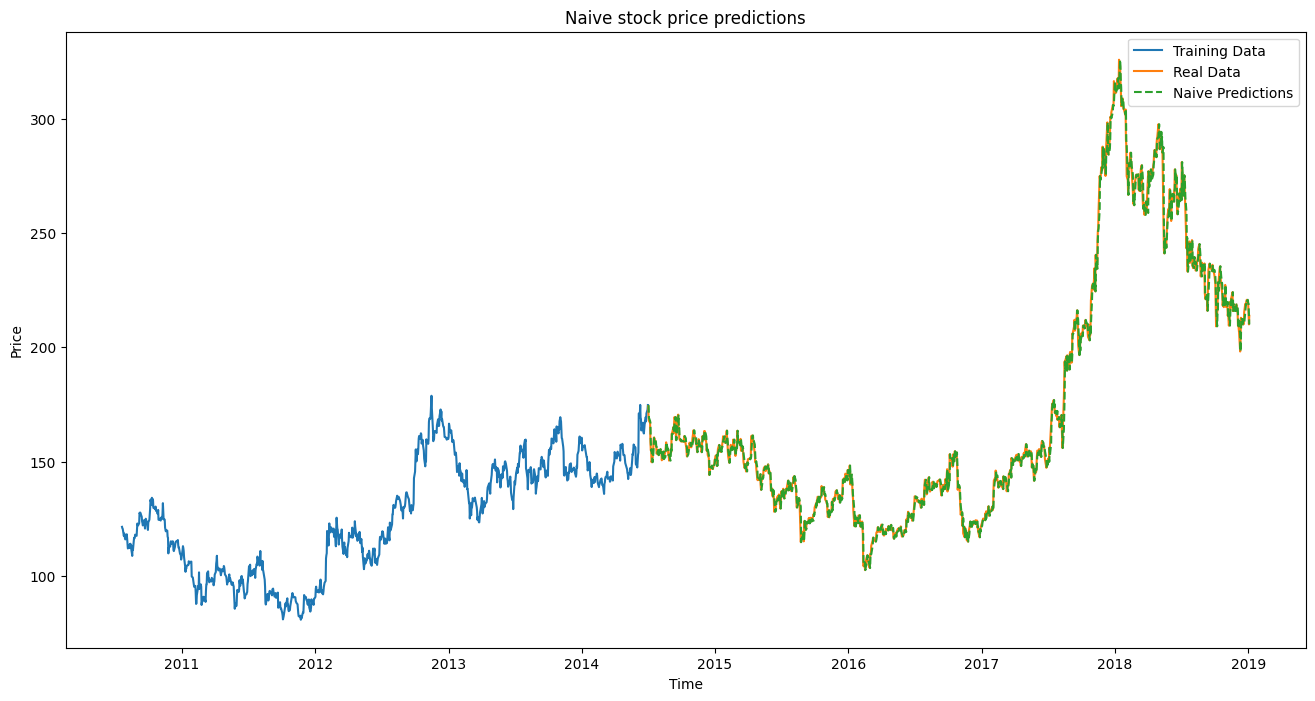
\includegraphics[width=0.95\textwidth]{figures/stock-prediction.png}
		\end{figure}
	}
	\only<2>{
		\begin{figure}[htbp]
			\centering
			\caption{如图为LSTM的预测结果}
			\label{fig:如图为LSTM的预测结果}
			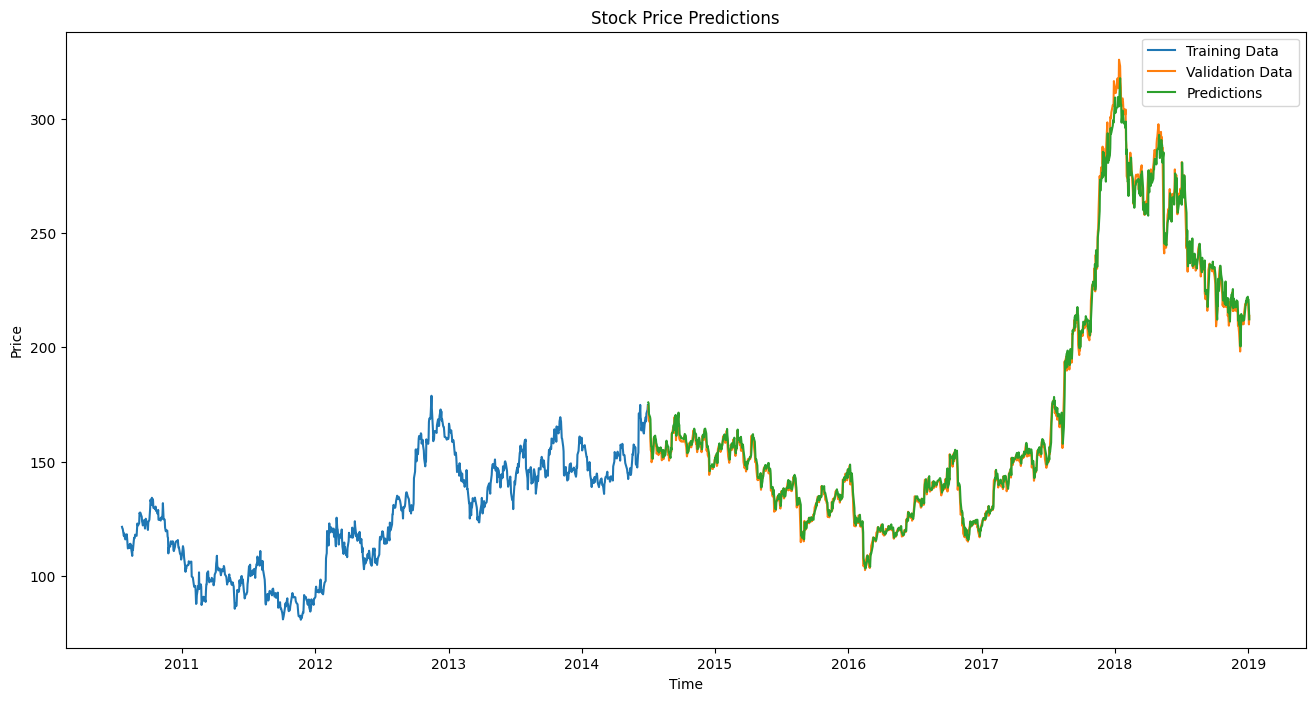
\includegraphics[width=0.95\textwidth]{figures/stock-prediction-lstm.png}
		\end{figure}
	}
\end{frame}

\subsection{模型结构}
\begin{frame}[fragile]{模型结构}
	\begin{minted}[breaklines,tabsize=4]{python}
lstm_model = Sequential()
lstm_model.add(
    LSTM(units=50, return_sequences=True, input_shape=(X_train.shape[1], 1))
)
lstm_model.add(Dropout(0.2))
lstm_model.add(LSTM(units=50))
lstm_model.add(Dropout(0.2))
lstm_model.add(Dense(1))

inputs = new_dataset[len(new_dataset) - len(valid_data) - 60 :].values
inputs = inputs.reshape(-1, 1)
inputs = scaler.transform(inputs)
print(inputs.shape)
	\end{minted}
\end{frame}

\begin{frame}[fragile]{模型结构}
	\begin{minted}[breaklines,tabsize=4]{python}
lstm_model.compile(loss="mean_squared_error", optimizer="adam")

# patience is the number of epochs to check for improvement
early_stop=EarlyStopping(monitor='val_loss', patience=10, verbose=1)

lstm_model.fit(X_train, y_train, epochs=100, batch_size=1, verbose=2, validation_split=0.2, callbacks=[early_stop])
	\end{minted}
\end{frame}

\begin{frame}[fragile]{模型结构}
	在本实验vs, 借助Keras搭建了一个LSTM神经网络. LSTM是为顺序数据特别设计的, 对于时
	序数据有良好预测性能, 且相比于RNN有效解决了长期记忆衰退问题的模型. 对其结构介绍如下.

	\begin{block}{输入层}
		模型期望输入数据有形状\mintinline[breaklines=true]{bash}|(X_train.shape[1], 1)|.
		这意味着每个训练样本应该是一个具有
		\mintinline[breaklines=true]{bash}|X_train.shape[1]|步的序列, 且在每一步只有一个特征.
	\end{block}
\end{frame}

\begin{frame}[fragile]{模型结构}
	\only<1>{
		\begin{block}{第一个LSTM层}
			\begin{itemize}
				\item 有50个神经元;
				\item 在tensorflow中, 设置
				      \mintinline[breaklines=true]{bash}|return_sequences=True|意味着这个LSTM层会将整
				      个序列传递给下一层, 对于堆栈的LSTM层是必要的.
			\end{itemize}
		\end{block}
	}
	\only<2>{
		\begin{block}{关于\mintinline[breaklines=true]{bash}|return_sequences|}
			LSTM层中的\mintinline[breaklines=true]{bash}|return_sequences|控制了LSTM输出的是序列还是整个序列的最后一个输出.

			设置\mintinline[breaklines=true]{bash}|return_sequences|为`True'或者`False'有特
			定的使用场景:

			\begin{enumerate}
				\item \mintinline[breaklines=true]{bash}|return_sequences=True|
				      \begin{itemize}
					      \item LSTM层会为输入序列中的每个时间步都产生一个输出, 意味着输出会和输入有相同的长度;
					      \item 将LSTM层堆叠的场景下这是必须的. 因为下一层需要和上一层期望相同长度的序列作为输入.
					      \item 如果进行的是seq2seq的预测, 则也应该使用这种方式.
				      \end{itemize}
				\item \mintinline[breaklines=true]{bash}|return_sequences=False|
				      \begin{itemize}
					      \item LSTM层会对整个输入序列产生一个单独的输出值. 这个只对应了最后一个时间步;
					      \item 当仅仅对于最后的预测结果感兴趣的时候, 这是合适的. 在许多seq2val的预测中采用这种方式.
					      \item 在一个全连接层之前, 通常也这样使用, 尤其是在分类或回归任务的模型中.
				      \end{itemize}
			\end{enumerate}
		\end{block}
	}
	\only<3>{
		\begin{block}{第一个Dropout层}
			该层随机设置20\%的输入单元为0, 这可以帮助避免过拟合.
		\end{block}
		\begin{block}{为什么在LSTM层之间使用Dropout层}
			\begin{itemize}
				\item Dropout层放在LSTM层之间的时候, 即对LSTM层的输出进行了dropout, 在训练时对其中的部
				      分值随机设置为0.
				\item Dropout可以有效避免过拟合, 尤其是在较小的数据集情况下(如本实验的数据集).
				\item 如果模型本身没有过拟合, 添加dropout不仅可能不会提供帮助, 反而可能降低模型
				      的表现. 因此, 需要监控验证表现并进行及时的调整.
			\end{itemize}
		\end{block}
	}
	\only<4>{\begin{block}{使用Dropout可能的缺点}
			\begin{itemize}
				\item 在RNN中使用dropout, 尤其是通过
				      \mintinline[breaklines=true]{bash}|recurrent_dropout|, 会延长训练时间, 因为在
				      Keras中对于\mintinline[breaklines=true]{bash}|recurrent_dropout|的实现关闭了对于
				      LSTM层的一些性能优化方法;
				\item 可能引入了过多的dropout, 这可能降低模型的学习能力. 在规范化模型和允许他从数据中学习之间应该取得一个平衡.
			\end{itemize}
		\end{block}}

	\only<5>{
		\begin{block}{第二个LSTM层}
			\begin{itemize}
				\item 具有50个单元;
				\item 因为后面没有后继的LSTM层, 因此
				      \mintinline[breaklines]{python3}|return_sequences|没有设置, 默认为False. 这意味着该层只会输出最后一个时间步的值.
			\end{itemize}
		\end{block}
	}
	\only<5>{\begin{block}{第二个Dropout层}
			仍旧20\%dropout率的Dropout层, 用来避免过拟合;
		\end{block}}

	\only<5>{\begin{block}{输出层}
			全连接层, 仅有一个神经元. 因为这里没有设置激活函数, 默认是线性激活函数, 使其适合回归任务.
		\end{block}}
\end{frame}

\subsection{训练方法}
\begin{frame}[fragile]{模型编译和训练}
	\begin{block}{编译}
		\begin{itemize}
			\item 模型使用平均平方差loss进行编译, 这对于回归任务是常用的选择. 使用的优化器是
			      `Adam', 对于许多深度学习任务这都是一个流行且高效的优化器.
		\end{itemize}
	\end{block}
	\begin{block}{提前停止回调}
		该回调函数监控了验证损失(\mintinline[breaklines]{python3}|val_loss|). 如果在10轮
		训练中验证loss没有提升(\mintinline[breaklines=true]{bash}|patience=10|), 训练会
		停止. 这可以帮助避免过拟合, 并且如果模型已经收敛, 可以帮助减少训练时间;
	\end{block}
	\begin{block}{模型训练}
		\begin{itemize}
			\item 模型训练了最多100轮, 批次大小为1. 意味着模型在每个样本之后都会更新参数.
			\item 20\%的数据用作验证数据.
			      (\mintinline[breaklines]{python3}|validation_split=0.2|).
			\item 使用了提前停止回调函数.
		\end{itemize}

	\end{block}
\end{frame}

\section{使用机器学习方法预测从泰坦尼克灾难中生存的可能}
\begin{frame}[fragile]{泰坦尼克}
	根据穿上人员的性别, 年龄, 职业等信息, 设计一种算法来预测泰坦尼克号上乘客的生存概
	率. 借助该问题, 学习使用`scikit-learn'库和xgboost等库的各种机器学习方法, 例如SVM
	支持向量机, 决策树, 线性模型, 朴素贝叶斯, 高斯过程和决策树等.
\end{frame}

\subsection{问题定义和特点}
\begin{frame}[fragile]{问题定义和特点}
	\only<1>{
		\begin{block}{问题描述}
			根据船上人员的各种特征,如性别、年龄、船票等级(Pclass)、上船地点(Embarked)、家庭成员数量、船票费用(Fare)以及其他相关信息,设计一种算法来预测泰坦尼克号上的乘客的生存概率。
		\end{block}
	}
	\only<2->{
		\begin{block}{问题的特点}
			对泰坦尼克生存预测任务中, 其问题的关键特点分析如下:

			\begin{enumerate}
				\item<only@2> \textbf{数据的复杂性与不完整性}
					- 数据集中存在大量缺失值,尤其是在'Age'和'Cabin'特征中。处理这些缺失值需要深思熟虑,因为简单的删除或填充可能会导致信息损失或引入偏见。

					- 存在一些杂乱的数据,例如在'Ticket'和'Name'特征中,这要求进行精细的数据清洗和特征工程。

				\item<only@2> \textbf{数据的不均衡性}
					- 大部分乘客在事故中未能生存。因此,我们面临的是一个不平衡分类问题,这可能会影响模型的评估指标和其对于生存和非生存类别的敏感性。

				\item<only@2> \textbf{特征的多样性}
					- 数据集中有数值、分类和文本特征。这意味着我们可能需要使用多种预处理技术来准备数据供模型使用。

					- 某些特征,如'Pclass'和'Sex',与生存率高度相关。但是,其他特征可能需要更深入的探索和工程化才能发挥其潜在价值。

				\item<only@3> \textbf{社会经济背景的影响}
					- 泰坦尼克号的生存率与社会阶层、性别和年龄等因素密切相关。例如,女性和儿童的生存率较高,而一等舱的乘客也有更高的生存机会。

					- 这提示我们,在特征工程和模型建立时,应考虑这些社会和经济背景。

				\item<only@3> \textbf{关于家庭的信息}
					- 'SibSp'和'Parch'两个特征提供了关于乘客家庭成员的信息。考虑到家庭成员可能一同行动(如逃生),这些特征可能与生存率有关。

					- 通过这些特征,可以派生出新的特征,如家庭大小或是否独自一人。
				\item<only@3> \textbf{隐藏信息的挖掘}
					- 例如,通过'Name'特征,可以提取出乘客的头衔,如`Mr', `Dr`等. 这与其社会地位、年龄和职业等相关,并间接影响其生存率。

			\end{enumerate}
		\end{block}
	}
\end{frame}

\subsection{数据特点}
\begin{frame}[fragile]{数据介绍}
	\begin{block}{数据介绍}
		数据中每个乘客有8个属性, 分别如下:
		\begin{enumerate}
			\item<only@1> `Survived`代表乘客是否存活
			\item<only@1> `PassengerID`和`Ticket`被假设为随机独立标识符, 对输出没有影响, 因此会被从分析中移除
			\item<only@1> `Pclass`代表票型, 并映射社会经济状态, 表示1 = 上层阶级, 2 = 中层阶级, 3 = 下层阶级;
			\item<only@1> `Name`是名字数据类型, 可能可以在特征工程中根据title判断性别, 从surname中家庭大小.

			\item<only@2> `Sex`和`Embarked`变量是命名数据类型. 会被转为dummy变量来进行数学计算.
			\item<only@2> `Age`和`Fare`变量是连续量化数据类型;
			\item<only@2> `SibSp`表示同在船上的兄弟姐妹的数量, `Parch`表示同在船上的父母孩子. 都是离散
				量化数据类型. 可以在特征工程中建立一个家庭大小, 是孤立的变量;
			\item `Cabin`变量是命名数据类型, 可以在特征工程中大致定位事故发生时在船上的位置, 以及根据等级判断接机. 然而, 由于有许多Null值, 该变量用处不大, 被排除在分析之外;
		\end{enumerate}
	\end{block}
\end{frame}

\begin{frame}[fragile]{使用的机器学习模型介绍}
	\begin{minted}[breaklines,tabsize=4]{python}
	# machine learning algorithms (MLA) selection and Initialization
MLA = [
    # ensemble methods
    ensemble.AdaBoostClassifier(),
    ensemble.BaggingClassifier(),
    ensemble.ExtraTreesClassifier(),
    ensemble.GradientBoostingClassifier(),
    ensemble.RandomForestClassifier(),
    # Gaussian Processes
    gaussian_process.GaussianProcessClassifier(),
    # GLM
    linear_model.LogisticRegressionCV(),
    linear_model.PassiveAggressiveClassifier(),
    linear_model.RidgeClassifierCV(),
    linear_model.SGDClassifier(),
    linear_model.Perceptron(),
	\end{minted}
\end{frame}

\begin{frame}[fragile]{使用的机器学习模型介绍}
	\begin{minted}[breaklines,tabsize=4]{python}
    # Naive Bayes
    naive_bayes.BernoulliNB(),
    naive_bayes.GaussianNB(),
    # Nearest Neighbor
    neighbors.KNeighborsClassifier(),
    # SVM
    svm.SVC(probability=True),
    svm.NuSVC(probability=True),
    svm.LinearSVC(),
    # Trees
    tree.DecisionTreeClassifier(),
    tree.ExtraTreeClassifier(),
    # Discriminant Analysis
    discriminant_analysis.LinearDiscriminantAnalysis(),
    discriminant_analysis.QuadraticDiscriminantAnalysis(),
    # XGBoost
    XGBClassifier(),
]
	\end{minted}
\end{frame}

\begin{frame}[fragile]{使用的机器学习模型介绍}
	\only<1>{\begin{block}{集成方法(Ensmble methods): 这些方法通常集合了多个模型(常常称为``基础学习者'')来提升泛化能力和鲁棒性}
			\begin{itemize}
				\item AdaBoostClassifier: 一个拟合一系列的弱学习者(通常是决策树)的自适应增强算法
				      . 每棵决策树都会纠正其前辈的错误.
				\item BaggingClassifier: 使用bagging
				      (Bootstrap Aggregating)来在数据集的随机子集上拟合一个分类器的多个实例. 子集是通
				      过替换获取的.
				\item ExtraTreesClassifier: 代表``Extremely Randomized Trees''. 像一个更加随机版
				      本的随机森林, 其中最好的划分从一个随机的子集和阈值中选取;
				\item GradientBoostingClassifier: 顺序添加预测器来纠正由前面的预测器做出的错误.
				      和AdaBoost不同, 该分类器专注于直接减少残差.
				\item RandomForestClassifier: 在训练中建立一个决策树`森林'. 每棵树都在数据和特征
				      的一个随机子集上训练. 预测被整合(对于回归任务取平均, 对于分类任务取多数投票).
			\end{itemize}
		\end{block}}
	\only<2>{\begin{block}{高斯过程}
			\begin{itemize}
				\item GaussianProcessClassifier: 一个用于回归和概率分类的非参数贝叶斯方法. 他在
				      函数上定义一个分布, 借助核技巧在高维空间中进行操作.
			\end{itemize}
		\end{block}
		\begin{block}{泛化线性模型}
			\begin{itemize}
				\item LogisticRegressionCV:具有用于自动参数调整的集成交叉验证的逻辑回归(用于二元分类).
				\item PassiveAggressiveClassifier: 一种适合大规模学习的在线学习算法, 被称为``被
				      动攻击'', 因为在正确分类时保持被动, 并在发生错误时变得攻击.
				\item RidgeClassifierCV: 使用L2正则化的线性分类器(对系数的平方幅度添加惩罚). 该版本包含集成的交叉验证.
				\item SGDClassifier: 线性分类器(像SVM和逻辑回归), 具有随机梯度下降(SGD)训练的线性分类器.
				\item Perceptron: 线性分类器的一种, 是一种监督二元分类算法.
			\end{itemize}
		\end{block}
	}
	\only<3>{\begin{block}{朴素贝叶斯}
			基于应用贝叶斯理论以及特征之间的强独立性假设.
			\begin{itemize}
				\item BernoulliNB: 二元数据使用. 假设特征是二元的.
				\item GaussianNB: 假设特征有高斯分布.
			\end{itemize}
		\end{block}
		\begin{block}{最近邻居}
			\begin{itemize}
				\item KNeighborsClassifier: 基于训练集中他的`k'个最近的邻居来分类一个样本.
			\end{itemize}
		\end{block}
		\begin{block}{支持向量机(SVM)}
			旨在找到最能将数据集划分为类别的超平面;
			\begin{itemize}
				\item SVC: 使用核技巧来变形输入数据, 然后识别最优的超平面;
				\item NuSVC: 和SVC类似, 但是使用一个参数`nu'来控制支持向量的数量.
				\item LinearSVC: 不是用核技巧的线性SVM.
			\end{itemize}
		\end{block}
	}
	\only<4>{
		\begin{block}{决策树}
			\begin{itemize}
				\item DecisionTreeClassifier: 构造一棵树, 其中每个节点都根据特征阈值作出决策. 分
				      割是根据熵或者基尼杂质(Gini impurity)等依据做出的;
				\item ExtraTreeClassifier: 类似决策树, 但是划分的更加随机.
			\end{itemize}
		\end{block}
		\begin{block}{判别分析: 用于分类和降维}
			\begin{itemize}
				\item LinearDiscriminantAnalysis, 线性判别分析(LDA): 假设每个类具有高斯分布, 并共享相同的协方差矩阵;
				\item QuadraticDiscriminantAnalysis, 二次判别分析(QDA): 与LDA类似, 但是允许每个类都有其协方差矩阵;
			\end{itemize}
		\end{block}
		\begin{block}{XGBoost}
			\begin{itemize}
				\item XGBClassifier:优化的梯度增强库. 代表eXtreme Gradient Boosting.以其速度和性能闻名.
			\end{itemize}
		\end{block}
	}
\end{frame}

\begin{frame}[fragile]{使用的机器学习模型介绍}
	\begin{minted}[breaklines,tabsize=4]{python}
cv_split = model_selection.ShuffleSplit(
    n_splits=10, test_size=0.3, train_size=0.6, random_state=0
)
# create table to compare MLA metrics
MLA_columns = [
    "MLA Name",
    "MLA Paramaters",
    "MLA Train Accuracy Mean",
    "MLA Test Accuracy Mean",
    "MLA Test Accuracy 3*STD",
    "MLA Time",
]
MLA_compare = pd.DataFrame(columns=MLA_columns)
# create table to compare MLA predictions
MLA_predict = data1[Target]
	\end{minted}
\end{frame}

\begin{frame}[fragile]{训练并进行预测}
	\begin{minted}[breaklines,tabsize=4]{python}
# index through MLA and save performance to table
row_index = 0
for alg in MLA:
    # set name and parameters
    MLA_name = alg.__class__.__name__
    MLA_compare.loc[row_index, "MLA Name"] = MLA_name
    MLA_compare.loc[row_index, "MLA Parameters"] = str(alg.get_params())

    # score model with cross validation
    cv_results = model_selection.cross_validate(
        alg,
        data1[data1_x_bin],
        data1[Target],
        cv=cv_split,
        return_train_score=True,
    )
	\end{minted}
\end{frame}

\begin{frame}[fragile]{训练并进行预测}
	\begin{minted}[breaklines,tabsize=4]{python}
    MLA_compare.loc[row_index, "MLA Time"] = cv_results["fit_time"].mean()
    MLA_compare.loc[row_index, "MLA Train Accuracy Mean"] = cv_results[
        "train_score"
    ].mean()
    MLA_compare.loc[row_index, "MLA Test Accuracy Mean"] = cv_results[
        "test_score"
    ].mean()
    # if this is a non-bias random sample, then +/-3 standard deviations(std)
    # from the mean, should statistically capture 99.7% of the subsets
    MLA_compare.loc[row_index, "MLA Test Accuracy 3*STD"] = (
        cv_results["test_score"].std() * 3
    )  # the worst that can happen

    # save MLA predictions
    alg.fit(data1[data1_x_bin], data1[Target])
    MLA_predict[MLA_name] = alg.predict(data1[data1_x_bin])

    row_index += 1

# print and sort table
MLA_compare.sort_values(
    by=["MLA Test Accuracy Mean"], ascending=False, inplace=True
)
MLA_compare
# MLA_predict
		\end{minted}
\end{frame}

\begin{frame}[fragile]{训练并进行预测}
	\only<1>{
		\begin{block}{交叉验证划分}
			借助`ShuffleSplit'方法订一个`cv\_split'这个交叉验证策略. 策略创建10个划分, 将数
			据中的60\%用于训练, 30\%用于测试. 该方法不是用整个数据集, 因为每个划分中有10\%的数据没有被使用.
		\end{block}
		\begin{block}{比较表}
			两个Pandas DataFrames(`MLA\_conpare'和`MLA\_predict')被初始化来存储每个算法的性能指标和预测.
		\end{block}
		\begin{block}{算法循环}
			在`MLA'列表中的每个算法都被循环经过, 不同的任务被执行:
			\begin{itemize}
				\item 算法名字和参数被保存;
				\item 算法在数据集上使用前面提到的划分策略进行交叉验证. 计算并存储训练准确度,测
				      试准确度, 拟合时间等指标.
				\item 算法在数据的一个子集上进行训练, 在同一个子集上进行预测. 这些预测会被保存, 在之后可视化训练结果的时候使用.
			\end{itemize}
		\end{block}
	}\only<2>{
		\begin{block}{结果}
			`MLA\_compare'DataFrame保存了性能指标, 基于测试准确度降序进行排序. 这使得找出表现最好的算法十分简单.
		\end{block}
	}
\end{frame}

\end{document}
